\documentclass[../main.tex]{subfiles}
% \begin{mdframed}[linecolor=blue]
% \end{mdframed}\medskip

\begin{document} %%%%%%%%%%%%%%%%%%%%%%%%%%%%%%%%%%%%%%%%%%%%%%%%%%%%%%%%%%%%
\section{Preguntas y Respuestas}

\subsection{El kernel}
    \begin{exercise}
        \textit{¿Qué es el Kelnel?}\\

        El kernel es la parte central del sistema operativo que gestiona los recursos del hardware y las interacciones con el software. 
        
        El kernel es responsable de ejecutar los programas, administrar la memoria, controlar los dispositivos de entrada y salida, y proporcionar seguridad y estabilidad al sistema.
    \end{exercise}

    \begin{exercise}
        \textit{¿Que es el ejecución directa?}\\

        Significa ejectar un programa directamente en la CPU. Beneficios: rapidez, Problemas: seguridad, confiabilidad, portabilidad.

        \underline{Limitar la ejecución directa:} 
        \begin{itemize}
            \item \textbf{Modo de operación dual:} es un mecanismo que proveen todas los procesadores, intercambia entre user mode y kernel mode.
            \item \textbf{Instrucciones Privilegiadas:} set de instrucciones que poseen cada modo de operación.
            \item \textbf{Proteccion de Memoria:} como la memoria es compartida, el SO debe poder configurar el hardware de forma tal que cada proceso pueda leer y escribir su propia porción de memoria.
            \item \textbf{Interrupciones por temporizador:} mecanismo le permita al kernel desalojar al proceso y volver a tomar el control del procesador.
        \end{itemize}
    \end{exercise}

\subsection{El proceso}

    \begin{exercise}
        \textit{Describa que es un proceso: qué abstrae, cómo lo hace, cuál es su estructura. Además explique el mecanismo por el cual el proceso cree tener la memoria completa de la máquina cuando en realidad solo tiene lo necesario para su funcionamiento.}\\

        Un proceso es \textbf{la ejecución de un programa} de aplicación con derechos restringidos; el proceso es la abstracción que provee el Kernel del sistema operativo para la ejecución protegida.

        Cuando se habla de derechos restringidos se está diciendo que está corriendo en una máquina donde hay dual mode, donde hay un kernel que tiene modo kernel y un set de instrucciones privilegiadas y este pobre tipo corre en el ring 3 con nada de privilegios.

        Cuando hace referencia a la abstracción se refiere a la virtualización del procesador (CPU), memoria y dispositivos de entrada/salida. Esta abstracción permite que varios procesos se ejecuten simultáneamente en la misma máquina, compartiendo los recursos físicos subyacentes de manera segura y asilada.

        La abstracción del proceso provee ejecución, aislamiento y protección.

        El mecanismo es la virtualización de memoria, que es una abstracción por la cual la memoria física puede ser compartida por diversos procesos.
        El sistema operativo asigna una cantidad limitada de memoria física a cada proceso, pero el proceso cree que tiene acceso a toda la memoria de la máquina.
        Cada proceso tiene su propio espacio de direcciones virtuales que es mapeado a la memoria física subyacente por el sistema operativo.
        La virtualización de memoria se logra mediante el uso de paginación y segmentación.
    \end{exercise}

    \begin{exercise}
        \textit{Cuál/cuáles mecanismos utiliza el kernel para garantizar el aislamiento entre procesos. Estos mecanismos están relacionados con el hardware, porque deben existir y donde se ve su funcionamiento.}\\

        El kernel utiliza la virtualización de memoria para garantizar el aislamiento entre procesos.
    \end{exercise}

    \begin{exercise}
        \textit{¿Que es la virtuaizacion?}\\

        Es crear una abstracción que haga que un dispositivo de hardware sea mucho más fácil de utilizar.
        Existen dos tipos de virtualización:
        \begin{itemize}
            \item \textbf{Virtualización de memoria:} Le hace creer al proceso que este tiene toda la memoria disponible.
                \begin{itemize}
                    \item Protección de Memoria: Memoria Virtual.
                    \item Traducción de Direcciones.
                \end{itemize} 
            \item \textbf{Virtualizacion de procesador:} Consiste en dar la ilusión de la existencia de un único procesador para cualquier programa que requiera de su uso.
            
            De esta forma, se prove:
            \begin{itemize}
                \item Simplicidad en la programación.
                \item Aislamiento frente a Fallas.
            \end{itemize}
        \end{itemize}
    \end{exercise}

    \begin{exercise}
        \textit{¿Cuales son los mecanismos de protección de memoria?}\\

        La memoria virtual es una asbtracción por al cual la memoria física puede ser compartida por diversos procesos.

        Un componente clave de la memoria virtual son las direcciones virtuales, con las direcciones virtuales, para cada proceso su memoria inicia en el mismo lugar, la dirección 0. 
        
        El hardware traduce la dirección virtual a una dirección física de memoria, se realiza por hardware (MMU).
    \end{exercise}

    \begin{exercise}
        \textit{¿Que es el address space?¿Que partes tiene?¿Para qué sirve?. Describa el/los mecanismos para crear un proceso en unix, sus sycalls, ejemplifique.}\\

        El address space es el espacio de direcciones virtuales que un proceso puede utilizar.  Está dividido en varias áreas: text, data, stack y heap.
        El propósito del address space es mantener separados los procesos y evitar que un proceso escriba en los datos de otro proceso.\\
        
        Para la creacion de un proceso:
        \begin{itemize}
            \item única forma es llamando a la system call \textit{fork}.
        \end{itemize}
    \end{exercise}

    \begin{exercise}
        \textit{¿Que es el stack ? Explique el mecanismo de funcionamiento del stack para x86 de la siguiente funcion int read(void *buff, size\_t num, int fd);.Como se pasan los parametros, direccion de retorno?.}\\

            El stack o pila es una estructura de datos que almacena información de forma temporal y ordenada, siguiendo el principio LIFO (Last In, First Out), es decir, el último en entrar es el primero en salir. El stack se usa para guardar los datos locales de una función, las direcciones de retorno de las llamadas a funciones y los parámetros que se pasan a las funciones.\\
            
            Para la función read(void *buff, size\_t num, int fd), que lee num bytes del archivo identificado por fd y los almacena en el buffer buff, se puede usar el stack para pasar los parámetros de la siguiente manera:
            \begin{itemize}
                \item Se empujan los parámetros al stack en orden inverso, es decir, primero fd, luego num y finalmente buff.
                \item Se llama a la función read con la instrucción call, que empuja la dirección de retorno al stack y salta a la etiqueta de la función.
                \item Dentro de la función read, se accede a los parámetros usando el registro ebp (base pointer) como referencia. El registro ebp se usa para guardar el valor del registro esp (stack pointer) al entrar en la función, y así poder acceder a los parámetros y variables locales sin importar cómo cambie el esp durante la ejecución de la función
                \item Se usa la convención cdecl para limpiar el stack después de la llamada a la función. Esta convención establece que el código que llama a la función es responsable de restaurar el esp al valor que tenía antes de empujar los parámetros. Esto se hace sumando al esp el tamaño total de los parámetros.
            \end{itemize}
            
            Un posible código en ensamblador x86 para este ejemplo sería:
            
            ; Código que llama a la función read ; Supongamos que fd = 3 (stdin), num = 100 y buff apunta a una zona de memoria reservada mov eax, 3 ; fd push eax ; empujar fd al stack mov eax, 100 ; num push eax ; empujar num al stack mov eax, buff ; buff push eax ; empujar buff al stack call read ; llamar a la función read add esp, 12 ; limpiar el stack (3 parámetros de 4 bytes cada uno)
            
            ; Código de la función read read: push ebp ; guardar el valor anterior de ebp mov ebp, esp ; copiar el valor de esp a ebp ; Ahora los parámetros se pueden acceder como [ebp+8], [ebp+12] y [ebp+16] ; Aquí iría el código para leer del archivo y escribir en el buffer ; usando las instrucciones syscall o int 80h mov esp, ebp ; restaurar el valor de esp pop ebp ; restaurar el valor de ebp ret ; retornar a la dirección guardada en el stack
    \end{exercise}
    
    \begin{exercise}
    \end{exercise}

\subsection{La Memoria}
    \begin{exercise}
        \textit{¿Que es la memoria virtual? ¿Qué mecanismos conoce, describa los tres que a usted le parezcan más relevantes?}\\

        La Memoria Virtual es un mecanismo de protección de memoria, provisto por el Hardware. La memoria virtual es una asbtracción por al cual la memoria física puede ser compartida por diversos procesos.
    \end{exercise}

        \begin{enumerate}
            \item 
                \textit{¿Que es la memoria virtual? ¿Qué mecanismos conoce, describa los tres que a usted le parezcan más relevantes?}\\
                
                \begin{itemize}
                    \item 
                        \textbf{La memoria segmentada} es una técnica de gestión de memoria que divide el espacio de memoria de un proceso en segmentos lógicos más pequeños y coherentes, en lugar de tratarlo como un espacio de memoria continuo y uniforme. Cada segmento representa una porción lógica de la memoria y puede contener diferentes tipos de datos, como código, datos, pila, tabla de símbolos, etc.

                        Cada segmento tiene un tamaño (Bound o registro límite o Segmento) y una dirección base (registro base) asociada. La dirección base indica la ubicación física donde comienza el segmento en la memoria física, mientras que el tamaño representa la longitud del segmento. En lugar de utilizar direcciones absolutas, se utilizan direcciones relativas dentro de cada segmento.
                        
                        La memoria segmentada ofrece varias ventajas. Permite una mayor flexibilidad en la asignación y el uso de memoria, ya que los segmentos pueden crecer o contraerse dinámicamente según las necesidades del proceso. También facilita el compartimiento de memoria entre diferentes procesos, ya que es posible compartir segmentos comunes entre ellos, lo que puede ahorrar espacio y mejorar la eficiencia.
                        
                        Sin embargo, la segmentación también puede presentar desafíos, como la fragmentación externa, que ocurre cuando hay espacios vacíos entre segmentos que no se pueden utilizar para almacenar otros segmentos. Esto puede llevar a un desperdicio de memoria. Además, la gestión de los segmentos y la traducción de direcciones pueden requerir una mayor complejidad en el hardware y el sistema operativo.
                        
                        En resumen, la memoria segmentada es una técnica de gestión de memoria que divide el espacio de memoria de un proceso en segmentos lógicos, lo que proporciona flexibilidad y compartición de memoria, pero puede implicar desafíos como la fragmentación externa.
                    \item 
                        \textbf{La memoria paginada} es una técnica de gestión de memoria en la que la memoria se divide en fragmentos de tamaño fijo llamados "page frames". En lugar de dividir la memoria en segmentos lógicos, como en la memoria segmentada, la memoria paginada la divide en páginas de tamaño uniforme. Cada página tiene un número de página virtual y una dirección física correspondiente.

                        El mecanismo de traducción de direcciones en la memoria paginada es similar al de la memoria segmentada. Cada proceso tiene una tabla de páginas (page table) que contiene entradas que mapean las páginas virtuales a las direcciones físicas de los page frames en la memoria física. Cuando un proceso accede a una dirección virtual, se utiliza la tabla de páginas para obtener la dirección física correspondiente.
                        
                        La dirección virtual consta de dos componentes: el número de página virtual y el desplazamiento (\textit{offset}) dentro de esa página. El número de página virtual se utiliza como índice en la tabla de páginas para obtener la dirección física del page frame correspondiente. Luego, se concatena el desplazamiento para obtener la dirección física completa.
                        
                        La memoria paginada ofrece varias ventajas, como una mayor eficiencia en la gestión de la memoria y la capacidad de compartir páginas entre procesos, lo que permite la memoria compartida. También facilita la protección de la memoria, ya que cada página se puede asignar permisos individuales de lectura, escritura y ejecución.
                        
                        Un aspecto importante de la memoria paginada es que proporciona una vista lógica de la memoria lineal para cada proceso, aunque las páginas pueden estar dispersas por toda la memoria física. Esto significa que las direcciones virtuales son continuas y lineales para el proceso, aunque las páginas físicas pueden estar ubicadas en diferentes ubicaciones físicas.
                        
                        En sistemas de paginación multinivel, como el utilizado en la arquitectura x86, se pueden utilizar múltiples niveles de tablas de páginas para gestionar direcciones virtuales más grandes de manera eficiente. Esto permite una mayor flexibilidad y eficiencia en la gestión de la memoria.
                        
                        En resumen, la memoria paginada es una técnica de gestión de memoria en la que la memoria se divide en páginas de tamaño fijo y se utiliza una tabla de páginas para traducir direcciones virtuales a direcciones físicas. Proporciona una vista lógica de la memoria lineal para cada proceso y ofrece ventajas como una gestión eficiente de la memoria y la capacidad de compartir páginas entre procesos.
                    \item 
                        \textbf{Paged Segmentation (Segmentación paginada)} es una combinación de la segmentación y la paginación. Consiste en dividir el espacio de direcciones lógicas en segmentos de tamaño variable, y luego dividir cada segmento en páginas de tamaño fijo. Cada segmento tiene una tabla de páginas asociada, que se almacena en una tabla de segmentos. El proceso de traducción de las direcciones lógicas a físicas es, primero se busca el segmento en la tabla de segmentos, luego se busca la página en la tabla de páginas del segmento, y finalmente concatena el frame de la oage table con el offset para obtener la dirección física completa.
                        \begin{itemize}
                            \item Reduce la fragmentación externa.
                            \item Mejora el rendimiento.
                            \item Proporciona un buen equilibrio entre flexibilidad y rendimiento
                        \end{itemize}
                \end{itemize}
            \item 
        \end{enumerate}

    \begin{exercise}
        \textit{Dado un sistema de paginación de 2 niveles de indirección, en el cual una v.a tiene un longitud de 32 bits, 10 bits para el PDI, 10 bits para el page table y finalmente 12 bits ara el offset. Indicar la cantidad de memoria en bytes máximas que pueden ocupar un proceso. justifique}\\
        
        En un sistema de paginación de dos niveles de indirección con una dirección virtual de 32 bits

        \begin{itemize}
            \item 10 bits para el índice del directorio de páginas (PDI)
            \item 10 bits para la tabla de páginas
            \item 12 bits para el desplazamiento
        \end{itemize}

        La cantidad máxima de memoria que puede ocupar un proceso se calcula de la siguiente manera:

        Primero, determinamos el tamaño de la página, que está dado por el desplazamiento. Como se utilizan 12 bits para el desplazamiento, el tamaño de la página es de $2^12$ bytes, o 4KB.

        Luego, determinamos el número total de entradas en la tabla de páginas, que está dado por el índice de la tabla de páginas. Como se utilizan 10 bits para el índice de la tabla de páginas (segment), hay $2^10$, o 1024, entradas en la tabla de páginas.

        Finalmente, determinamos el número total de tablas de páginas, que está dado por el índice del directorio de páginas. Como se utilizan 10 bits para el índice del directorio de páginas, hay $2^10$, o 1024, tablas de páginas.

        Por lo tanto, la cantidad máxima de memoria que puede ocupar un proceso es el tamaño de la página multiplicado por el número total de entradas en la tabla de páginas multiplicado por el número total de tablas de páginas. Esto es, 4 KB * 1024 * 1024, o 4 GB. Por lo tanto, un proceso puede ocupar un máximo de 4 GB de memoria en este sistema de paginación.\\

        Convertir \(2^{32}\) a gigabytes (GB):

        Cuando decimos \(2^{32}\), estamos utilizando notación exponencial. En este caso, \(2^{32}\) significa "2 elevado a la potencia de 32". Para convertir esto a bytes, recordamos que 1 byte es igual a \(2^0\), 1 kilobyte (KB) es igual a \(2^{10}\) bytes, 1 megabyte (MB) es igual a \(2^{20}\) bytes, y 1 gigabyte (GB) es igual a \(2^{30}\) bytes.

        Entonces, para convertir \(2^{32}\) a gigabytes, dividimos \(2^{32}\) por \(2^{30}\):

        \[ \frac{2^{32}}{2^{30}} = 2^{32-30} = 2^2 = 4 \]

        Por lo tanto, \(2^{32}\) bytes es igual a 4 gigabytes. En el contexto de la memoria de un sistema informático, esta es la razón por la cual a menudo escuchamos que un sistema de 32 bits puede direccionar hasta 4 GB de memoria.
    \end{exercise}

\subsection{Concurrencia}
    \begin{enumerate}
        \item 
            \textbf{¿Que es un thread?. Use su API para crear un programa que use 5 thread para incrementar una  variable compartida por todos en 7 unidades/thread hasta llegar a 100}\\
            Un thread es una secuencia de ejecución atómica que representa una tarea planificable de ejecución. También una secuencia independiente de instrucciones ejecutándose dentro de un programa.
            
            \begin{lstlisting}[language=Python, caption=hola mundo.]
                #include <stdio.h>
    
                int main() {
                printf("hello, world\n");
                }
            \end{lstlisting}
        \item
    \end{enumerate}

\subsection{File System}
    \begin{exercise}
        El superbloque de un sistema de archivos indica que el inodo correspondiente al directorio raiz es el \#43. En la siguiente secuencia de comandos y siempre partiendo de ese directorio raiz, se pide indicar  la cantidad de inodos y bloquies de datos a los que se precisa acceder (leer) para resolver la ruta dada a cat(1) o stat(1)
        
        \begin{lstlisting}[language=c, caption=hola mundo.]
# mkdir /dir /dir/s /dir/s/w
# touch /dir/x /dir/s/y
# stat /dir/s/w/x   // Inodos: ......   Bloque Datos: ......
# stat /dir/s/y     // Inodos: ......   Bloque Datos: ......

# ln /dir/s/x  /dir/h
# ln -s /dir/s/y /dir/y
# cat /dir/h        // Inodos: ......   Bloque Datos: ......
# cat /dir/y        // Inodos: ......   Bloque Datos: ......
        \end{lstlisting}

        Ayuda: todos los directorios ocupan un bloque. La idea es que describan como stat llega a los archivos.

        \begin{answer}
            Ver la Figura \ref{fig:file-system}, también se puede ver la carpeta "markodown-chatGPT".

            Como dice desde el directorio raíz. 
            \begin{itemize}
                \item \textbf{stat /dir/s/y:} Entonces se accede al inode del directorio "dir" (1 inode) se accede a su bloque (1 bloque) que contiene el directorio "s", se accede al inode del directorio "s" (1 inode) se accede a su bloque (1 bloque), que contiene el directorio "w", se accede al inode del directorio "w" (1 inode) se accede a su bloque (1 bloque), está vacío porque no se creó ningún archivo. Entonces: 3 inodes y 3 bloques
                \item \textbf{stat /dir/s/y:} Para este caso se da lo mismo que el anterior, pero en vez de acceder al inode del directorio "w" se accede al inode del archivo "y" (1 inode) se accede a su bloque (1 bloque). Entonces: 3 inodes y 3 bloques.
                \item \textbf{cat /dir/h:} Suponiendo que el comando "ln /dir/s/x  /dir/h" no falle, sería 1 inode y 1 bloque. Pero como falla, no se crea el hardlink, entonces no se accede a ningún inode ni bloque.
                \item \textbf{cat /dir/y:} Sería 2 inode y 2 bloque. Por que es un symlink. Se accede al inode del directorio "dir" (1 inode) se accede a su bloque (1 bloque) que contiene el symlink "y", se accede al inode de "y" que esta en el directorio "s" y luego a su bloque (1 bloque). Entonces: 2 inodes y 2 bloques.
            \end{itemize}
        \end{answer}
        \label{ex:file-system}
    \end{exercise}

    \begin{figure}[ht]
        \centering
        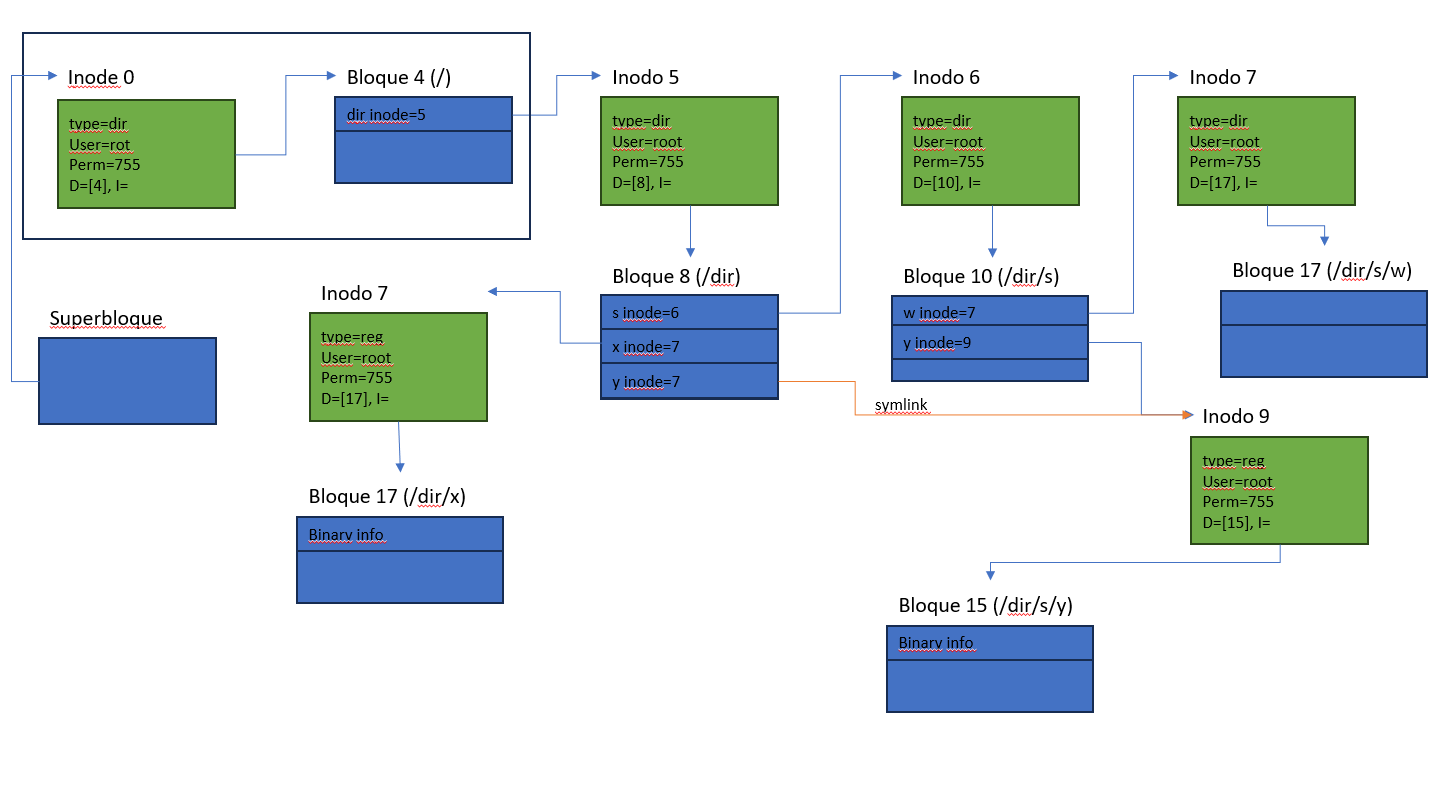
\includegraphics[scale=0.3]{../images/file-system.png}
        \label{fig:file-system}
        \caption{File System de la respuesta del Ejercicio \ref{ex:file-system} \href{https://fiubaar-my.sharepoint.com/:p:/g/personal/lcondoriz_fi_uba_ar/ERIlPc9eeJNOg9fCVzz2cjgBsjhy15nYJswfVTfWUNNcTg?e=KJvO2T}{PowerPoint}}
    \end{figure}

    \begin{exercise}
        Describir que es un File System.
        \begin{answer}
            Un File System es un conjunto de estructuras de datos y algoritmos que permiten la administración de archivos en un sistema operativo.
            \begin{itemize}
                \item \textbf{Superbloque:} contiene información sobre el sistema de archivos, como el tamaño del sistema de archivos, el tamaño de los bloques, el número de bloques, el número de inodos, etc. Apunta al inodo del directorio raíz.
            \end{itemize}
        \end{answer}
    \end{exercise}

    \begin{exercise}
        Sea un disco que posee 2049 bloques de 4KiB y un sistema operativo cuyos i-nodos son de 512 bytes. Definir un sistema de archivos FFS. Explique las decisiones tomadas.

        \begin{answer}
            La estructura de un File System es la siguiente:
            \begin{itemize}
                \item \textbf{Superbloque:} apunta al inodo del directorio raíz.
                \item \textbf{bitmap inodos:} indica qué inodos están libres y cuáles están ocupados.
                \item \textbf{bitmap bloques:} indica qué bloques están libres y cuáles están ocupados.
                \item \textbf{inodos:} contiene información sobre los archivos, como el tamaño, los permisos, etc.
                \item \textbf{bloques de datos:} contienen los datos de los archivos.
            \end{itemize}
            Pra el superbloque (1 bloque = 4KiB), bitmap inodos (1 bloque = 4KiB), bitmap bloques (1 bloque = 4KiB) y los inodos (512 bloques), data región (1534 bloques).\\

            Determinamos cuantos inodos caben en un bloque de 4KiB = 4094 bytes: 4096 bytes / 512 bytes = 8 inodos.

            Cantidad máxima de archivos/directorios: 512 bloques * 8 inodos/bloque = 4096 inodos.\\

            Cantidad de los bloques de datos: 1534 bloques * 4KiB = 6136 KiB = 6 MiB.
   
        \end{answer}
    \end{exercise}

    \begin{exercise}
        Los nombres de archivo no se almacenan en los i-nodos, sino en bloques de datos. ¿Por qué?.

        Este diseño posibilita la implementación de enlaces de tipo, marque la opción correcta:
        \begin{itemize}
            \item symlink
            \item hardlink
            \item ambos \checkmark
            \item ninguno  
        \end{itemize}

        \begin{answer}
            Esta elección permite tanto enlaces simbólicos (symlink) como enlaces duros (hardlink). Los enlaces simbólicos son referencias a otros archivos por su nombre, mientras que los enlaces duros son múltiples entradas de directorio que apuntan al mismo inodo (y por lo tanto, al mismo conjunto de bloques de datos). Ambos tipos de enlaces comparten el mismo conjunto de bloques de datos, pero tienen diferentes inodos y nombres de archivo. Este diseño proporciona flexibilidad y eficiencia en la gestión de enlaces en el sistema de archivos. Ver Figura \ref{fig:hard-sym-link}.
        \end{answer}
        \label{ex:hard-sym-link}
    \end{exercise}

    \begin{figure}[ht]
        \centering
        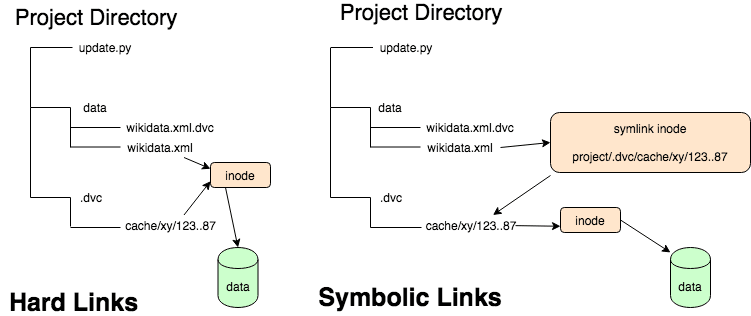
\includegraphics[scale=0.45]{../images/hard-sym-link.png}
        \label{fig:hard-sym-link}
        \caption{Hardlink y Symlink. Ejercicio \ref{ex:hard-sym-link}}
    \end{figure}

    \begin{exercise}
        ¿Qué es un inodo? ¿Qué información contiene?
    \end{exercise}

    \begin{exercise}
        Se tiene un file system basado en i-nodos con la siguientes características:
        \begin{itemize}
            \item Los bloques son de 1 kiB (1024 bytes) $[2^10]$.
            \item EI tamaño de un i-nodo es de 64 bytes $[2^6]$.
        \end{itemize}
        La distribución de los bloques es: 
        \begin{itemize}
            \item EI bloque 0 es el boot\_block.
            \item EI bloque 1 es el superblock.
            \item EI bloque 2 es el isnode\_bitmap.
            \item EI bloque 3 es el block-bitmap.
            \item Hay 126 bloques dedicados a la i-nodo table.
            \item Hay 128 bloques dedicados a datos.
        \end{itemize}
        Dada la siguiente información de la tabla de i-nodos y el contenido de los bloques de datos. indicar:
        \begin{enumerate}
            \item ¿Qué se mostraria en pantalla o que equivale ejecutar \textit{ls home/dato} y \textit{ls home/juan}?
            \item Indicar la secuencia de operaciones (lecturas de bloque blkrd indicando la numeración relativa a la sección de Ánodos o datos: y la numeración dentro del sistema entero). que se realizan para acceder al archivo \textit{ls home/dato/start.sh}. Indicar para cada bloque leído qué información contiene y qué parte resulta relevante.
            \item ¿Hay algún archivo que tenga más de una referencia (hard link)? ¿Qué syscall o comando unix usaría para borrar este tipo de archivos?
        \end{enumerate}

        \begin{answer}
            Ver el \href{https://fiubaar-my.sharepoint.com/:p:/g/personal/lcondoriz_fi_uba_ar/ERIlPc9eeJNOg9fCVzz2cjgBsjhy15nYJswfVTfWUNNcTg?e=KJvO2T}{PowerPoint} diapositiva 2. El enuciado esta en la carpeta parciales.\\

            \begin{enumerate}
                \item \textit{ls home/dato}: Al ejectarse el file system comienza accediendo al superbloque, el cual apunta al inodo del direcrorio raíz (/). Una vez accedido al inodo del directorio raíz, se accede al bloque de datos, tiene el bloque 0 y 1, en el bloque 1 se encuantra el directorio home. El directorio home tiene un inodo 5, se accede al inodo 5, se accede al bloque de datos, tiene bloque directos: 7 y 9 y indirectos: 0 (Block ptr). El block ptr = 0, me dice que ingrese al data block 0, ahi va estar "dato". Me manda al inode 11, y luego block ptr = 9, me manda al data block 9. En tonces com \textit{ls home/dato} me muestra "jos.c star.c". 
            \end{enumerate}
        \end{answer}
    \end{exercise}

    
\subsection{Definiciones sueltas}
    El sistema operativo tiene que poder configurar el hardware de forma tal que cada proceso pueda leer y escribir solo su propia memoria.

\end{document}  %%%%%%%%%%%%%%%%%%%%%%%%%%%%%%%%%%%%%%%%%%%%%%%%%%%%%%%%%%%%%